\tikzset{every picture/.style={line width=0.75pt}}   

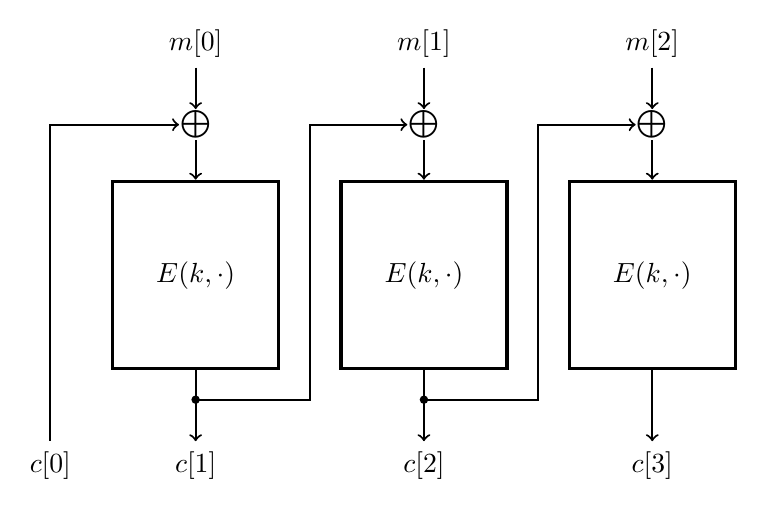
\begin{tikzpicture}[x=0.75pt,y=0.75pt,yscale=-1,xscale=1]

\draw  [line width=1.2]  (45,75) -- (125,75) -- (125,165) -- (45,165) -- cycle ;
\draw  [line width=1.2]  (265,75) -- (345,75) -- (345,165) -- (265,165) -- cycle ;
\draw  [line width=1.2]  (155,75) -- (235,75) -- (235,165) -- (155,165) -- cycle ;

\draw  [->]  (85,20) -- (85,40) ;
\draw  [->]  (195,20) -- (195,40) ;
\draw  [->]  (305,20) -- (305,40) ;

\draw  [->]  (85,55) -- (85,74) ;
\draw  [->]  (195,55) -- (195,74) ;
\draw  [->]  (305,55) -- (305,74) ;

\draw  [->]  (85,165) -- (85,200) ;
\draw  [->]  (195,165) -- (195,200) ;
\draw  [->]  (305,165) -- (305,200) ;

\draw  [<-]  (77,47.5) -- (15,47.5) -- (15,200) ;
\draw  [<-]  (187,47.5) -- (140,47.5) -- (140,180) -- (85,180) ;
\draw  [<-]  (297,47.5) -- (250,47.5) -- (250,180) -- (195,180) ;

\draw  [fill={rgb, 255:red, 0; green, 0; blue, 0 }  ,fill opacity=1 ] (83.5,180) .. controls (83.5,179.17) and (84.17,178.5) .. (85,178.5) .. controls (85.83,178.5) and (86.5,179.17) .. (86.5,180) .. controls (86.5,180.83) and (85.83,181.5) .. (85,181.5) .. controls (84.17,181.5) and (83.5,180.83) .. (83.5,180) -- cycle ;
\draw  [fill={rgb, 255:red, 0; green, 0; blue, 0 }  ,fill opacity=1 ] (193.5,180) .. controls (193.5,179.17) and (194.17,178.5) .. (195,178.5) .. controls (195.83,178.5) and (196.5,179.17) .. (196.5,180) .. controls (196.5,180.83) and (195.83,181.5) .. (195,181.5) .. controls (194.17,181.5) and (193.5,180.83) .. (193.5,180) -- cycle ;

\draw (85,120) node    {$E( k,\cdot )$};
\draw (85,16.6) node [anchor=south] [inner sep=0.75pt]    {$m[ 0]$};
\draw (15,203.4) node [anchor=north] [inner sep=0.75pt]    {$c[ 0]$};
\draw (195,120) node    {$E( k,\cdot )$};
\draw (195,16.6) node [anchor=south] [inner sep=0.75pt]    {$m[ 1]$};
\draw (85,203.4) node [anchor=north] [inner sep=0.75pt]    {$c[ 1]$};
\draw (305,120) node    {$E( k,\cdot )$};
\draw (305,16.6) node [anchor=south] [inner sep=0.75pt]    {$m[ 2]$};
\draw (195,203.4) node [anchor=north] [inner sep=0.75pt]    {$c[ 2]$};
\draw (85,47.5) node    {$\bigoplus $};
\draw (195,47.5) node    {$\bigoplus $};
\draw (305,47.5) node    {$\bigoplus $};
\draw (305,203.4) node [anchor=north] [inner sep=0.75pt]    {$c[ 3]$};

\end{tikzpicture}